\item \textbf{{[}NYJC/PRELIM/9569/2020/P1/Q5{]} }

Athletes, who are members of teams, compete in running events, which
are held at fixtures throughout the year. For example, athlete 15
might compete in the Girls\textquoteright{} 1500m Under 18 race in
the fixture at National Stadium on 12 September 2020.

A relational database is used to store the details of which athletes
enter each event at each fixture. The relations used in the database
are shown in \textbf{Figure 5}.
\noindent \begin{center}
\textbf{Figure 5}
\par\end{center}

\texttt{Athlete(}\texttt{\uline{AthleteID}}\texttt{, Surname, Forename,
DateOfBirth, Gender, TeamName) }

\texttt{EventType(}\texttt{\uline{EventTypeID}}\texttt{, Gender,
Distance, AgeGroup) }

\texttt{Fixture(}\texttt{\uline{FixtureID}}\texttt{, FixtureDate,
LocationName) }

\texttt{EventAtFixture(}\texttt{\uline{FixtureID}}\texttt{, }\texttt{\uline{EventTypeID}}\texttt{) }

\texttt{EventEntry(}\texttt{\uline{FixtureID}}\texttt{, }\texttt{\uline{EventTypeID}}\texttt{,
}\texttt{\uline{AthleteID}}\texttt{) }
\begin{itemize}
\item Each \texttt{Athlete}, \texttt{EventType} and \texttt{Fixture} is
identified by a unique identity number, for example \texttt{AthleteID}
for athletes. 
\item An \texttt{EventType} is a type of event, such as Boys\textquoteright{}
100m Under 15 race. 
\item If an athlete wants to take part in an event at a particular fixture,
then an entry is created in the \texttt{EventEntry} relation to represent
this. 
\end{itemize}
\textbf{Figure 6} shows an incomplete entity-relationship diagram
for part of the database. 
\noindent \begin{center}
\textbf{Figure 6}
\par\end{center}

\begin{center}
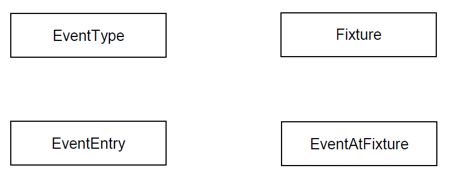
\includegraphics[width=0.5\paperwidth]{C:/Users/Admin/Desktop/Github/question_bank/LyX/static/img/9569-NYJC-2020-P1-Q5}
\par\end{center}
\begin{enumerate}
\item Copy and draw lines on \textbf{Figure 6} to show the degree of any
\textbf{three} relationships that exist between the four entities
shown. {[}3{]}
\item The following SQL statement is intended to make a table to represent
the Athlete relation. The statement contains some errors. 
\noindent \begin{center}
\textbf{Figure 7}
\par\end{center}

\noindent %
\noindent\begin{minipage}[t]{1\columnwidth}%
\texttt{CREATE TABLE Athlete ( }

\texttt{\qquad{}PRIMARY KEY AthleteID, }

\texttt{\qquad{}VARCHAR(50) Surname, }

\texttt{\qquad{}VARCHAR(30) Forename, }

\texttt{\qquad{}DATE DateOfBirth, }

\texttt{\qquad{}VARCHAR(6) Gender, }

\texttt{\qquad{}VARCHAR(30) TeamName }

\texttt{) }%
\end{minipage}

You may assume that all of the data types used in \textbf{Figure 7}
are valid and the field lengths are appropriate. State \textbf{two}
errors that have been made. \hfill{}{[}2{]}
\item State two reasons why database designs, such as this one, are usually
normalised. \hfill{}{[}2{]}
\item A list is to be produced of the names of all athletes who are competing
in the fixture that is taking place on 17/09/20. The list must include
the \texttt{Surname}, \texttt{Forename} and \texttt{DateOfBirth} of
these athletes and no other details. The list should be presented
in alphabetical order by Surname. With reference to the database design
shown in Figure 3, write an SQL query to produce the list. \hfill{}{[}5{]}
\item An IT consultant is suggesting changing to the use of a NoSQL database
instead.
\begin{enumerate}
\item Describe two advantages that a NoSQL database have over a SQL database.
\hfill{} {[}4{]}
\item Explain with reasons if you agree or disagree with making the change.
\hfill{}{[}2{]}
\end{enumerate}
\end{enumerate}